\subsection{On the Role of Architecture}
\begin{frame}{\insertsubsection}
	\begin{fancycolumns}
		\centering
		\pic[height=60mm]{misc/ulm-muenster} % TODO remove and replace by other building?
	\end{fancycolumns}
\end{frame}

\begin{frame}{Architecture Bridges the Gap}
	\begin{fancycolumns}[columns=3,animation=none]
		\uncover<4->{
			\begin{example}{}
				Large software systems \ldots
				\begin{itemize}
					\item have numerous requirements
					\item require many developers
					\item need separation of concerns\\\deutsch{Trennung von Belangen}
				\end{itemize}
			\end{example}
		}
		\nextcolumn
		\nextcolumn
		\uncover<3>{
			\begin{note}{}
				\mycite{Weeks of coding can save you hours of planning.}\mysource{anon}
			\end{note}
		}
	\end{fancycolumns}
	\begin{tikzpicture}[xscale=4.95]
		\node[label=below:Requirements] (req) at (0,0) {\pic[height=2.5cm]{architecture/requirements}};
		\only<2-3,6->{\node[label=below:Implementation] (code) at (2,0) {\pic[height=2.5cm]{architecture/source-code}};}
		%\only<2>{\node[label=below:Softwarearchitektur] (swa) at (.95,0) {\includegraphics[height=1.9cm]{component-diagram}};}
		\only<5->{
			\draw[->,line width=5pt,gray] (req) -- (code);
			\node[label=below:Software Architecture] (swa) at (.95,0) {\pic[height=2.5cm]{architecture/component-diagram-large}};
		}
	\end{tikzpicture}
\end{frame}

\subsection{Recap: Process Models}
\begin{frame}[10]{\insertsubsection}
	\begin{fancycolumns}[widths={45}]
		\diagramWaterfallModel
		\nextcolumn
		\diagramVModel
	\end{fancycolumns}
\end{frame}

\subsection{Software Architecture}
\begin{frame}{\insertsubsection\ \mytitlesource{\sommerville}}
	\begin{fancycolumns}[keep]
		\begin{definition}{Architectural Design \deutsch{Architekturentwurf}}
			\mycite{\emph{Architectural design} is a creative process in which you design a system organization that will satisfy the functional and non-functional requirements of a system.}
		\end{definition}
		\pause
		\begin{definition}{Software Architecture}
			\mycite{A \emph{software architecture} is a description of how a software system is organized. Properties of a system such as performance, security, and availability are influenced by the architecture used.}
		\end{definition}
		\nextcolumn
		\pause
		\begin{example}{In Practice:}
			\mycite{You might propose an abstract system architecture where you associate groups of system functions or features with large-scale components or subsystems. You then use this decomposition to discuss the requirements and more detailed features of the system with stakeholders.}
		\end{example}
	\end{fancycolumns}
\end{frame}

\xkcdframe{2347}

\subsection{3 Goals of Software Architecture}
\begin{frame}{\insertsubsection\ \normalsize[\sommerville]}
	\begin{fancycolumns}[columns=1] % hack to make mindmap visible in dark mode
		{\tikz[grow cyclic,
			mindmap, every node/.style=concept,concept color=red!20!background,
			%text width=20mm,align=flush center,
			level 1/.append style={level distance=27mm,sibling angle=360/3}]
			\node {Goals of Software Architectures}
			[clockwise from=90]
			child { node {communication of stakeholders} }
			child { node {meet critical requirements} }
			child { node {support software reuse} }
			;}
	\end{fancycolumns}
\end{frame}

\subsection{4 Views in Software Architecture}
\begin{frame}{\insertsubsection\ \normalsize[\sommerville]}
	\begin{fancycolumns}[keep]
		{\tikz[grow cyclic,
			mindmap, every node/.style=concept,concept color=blue!20!background,
			%text width=20mm,align=flush center,
			level 1/.append style={level distance=27mm,sibling angle=360/4}]
			\node {Architectural Views}
			child { node {logical view} }
			child { node {process view} }
			child { node {development view} }
			child { node {physical view} }
			;}
		\nextcolumn
		\begin{definition}{\sommerville:}
			\small
			\mycite{\uncover<2->{A \emph{logical view}, which shows the key abstractions in the system as objects or object classes. It should be possible to relate the system requirements to entities in this logical view.}
				
				\uncover<3->{A \emph{process view}, which shows how, at runtime, the system is composed of interacting processes. This view is useful for making judgments about non-functional system characteristics such as performance and availability.}
				
				\uncover<4->{A \emph{development view}, which shows how the software is decomposed for development; that is, it shows the breakdown of the software into components that are implemented by a single developer or development team. This view is useful for software managers and programmers.}
				
				\uncover<5->{A \emph{physical view}, which shows the system hardware and how software components are distributed across the processors in the system. This view is useful for systems engineers planning a system deployment.}}
		\end{definition}
	\end{fancycolumns}
\end{frame}

\subsection{Conway's Law}
\begin{frame}
	\begin{fancycolumns}[height=8.5cm]
		\pic[width=\linewidth,trim=0 50 0 0,clip]{people/melvin-conway}
		\vspace{-7mm}
		
		\begin{note}{Melvin E. Conway (1968) \mysource{\href{http://www.melconway.com/Home/Committees_Paper.html}{melconway.com}}}
			Conway's Law: \mycite{Any organization that designs a system [...] will produce a design whose structure is a copy of the organization's communication structure.}
		\end{note}
	\end{fancycolumns}
\end{frame}
